\documentclass[12pt]{article}
\usepackage{amsmath, amssymb, amsthm, enumerate, graphicx}
\usepackage[usenames,dvipsnames]{color}
\usepackage{bm}
\usepackage[colorlinks=true,urlcolor=blue]{hyperref}
\usepackage{geometry}
\geometry{margin=1in}
\usepackage{float}
\usepackage{graphics}
\setlength{\marginparwidth}{2.15cm}
\usepackage{booktabs}
\usepackage{enumitem}
\usepackage{epsfig}
\usepackage{setspace}
\usepackage{parskip}
\usepackage[normalem]{ulem}
\usepackage{tikz}
\usetikzlibrary{positioning, arrows, automata}
\usepackage{pgfplots}
\pgfplotsset{compat=newest}
\usepackage[font=scriptsize]{subcaption}
\usepackage{float}
\usepackage[]{algorithm2e}
\usepackage{environ}
\usepackage{bbm}
\usepackage{graphicx}
\usepackage{titling}
\usepackage{url}
\usepackage{xcolor}
\usepackage{lipsum}
\usepackage{lastpage}
\usepackage[colorlinks=true,urlcolor=blue]{hyperref}
\usepackage{multicol}
\usepackage{tabularx}
\usepackage{comment}
\usepackage[utf8]{inputenc}
\usepackage{amssymb}
\usepackage{setspace}
\usepackage{marvosym}
\usepackage{wrapfig}
\usepackage{datetime}
\usepackage[many]{tcolorbox}
\usepackage{array}
\usepackage{multirow}
\usepackage{wasysym}
\usepackage{cancel}
\usepackage{cprotect}
\usepackage{listings}
\usepackage{color}
\usetikzlibrary{matrix}

\newcommand{\blackcircle}{\tikz\draw[black,fill=black] (0,0) circle (1ex);}
\renewcommand{\circle}{\tikz\draw[black] (0,0) circle (1ex);}

\newtcolorbox[]{solution}[1][]{%
    breakable,
    enhanced,
    colback=white,
    title=Solution,
    #1
}


% SOLUTION environment
% \NewEnviron{soln}{
% \leavevmode\color{red}\ignorespaces \textbf{Solution} \BODY }{}
\NewEnviron{soln}[1]{
\begin{solution}[#1]
\leavevmode\color{red}\ignorespaces \BODY 
\end{solution}
}{}

% QUESTION AUTHORS environment
\NewEnviron{qauthor}{
\leavevmode\color{blue}\ignorespaces \textbf{Author} \BODY}{}

% SOLUTION environment
\NewEnviron{qlearningobjective}{
\leavevmode\color{blue}\ignorespaces \textbf{Learning Objective } \BODY }{}

% TO ONLY SHOW HOMEWORK QUESTIONS, include following (else comment out):
\RenewEnviron{soln}[1]{\begin{solution}[#1] \BODY \end{solution}}  % Use this for the handout tex
\RenewEnviron{qauthor}{}
\RenewEnviron{qlearningobjective}{}

%\newcommand{\norm}[1]{\lVert #1 \rVert}
%\newcommand{\st}{\mathrm{s.t.}}

\makeatletter
\newcommand{\removelatexerror}{\let\@latex@error\@gobble}
\makeatother

\newcommand{\argmax}{\mathop{\mathrm{argmax}}}
\newcommand{\argmin}{\mathop{\mathrm{argmin}}}

%%%%%%%%%%%%%%%%%%%%%%%%%%%%%%%%%%%%%%%%%%%
% Custom Math                             %
%%%%%%%%%%%%%%%%%%%%%%%%%%%%%%%%%%%%%%%%%%%


%%%%%%%%%%%%%%%%%%%%%%%%%%%%%%%%%%%%%%%%%%%
% Custom box for highlights               %
%%%%%%%%%%%%%%%%%%%%%%%%%%%%%%%%%%%%%%%%%%%

% Define box and box title style
\tikzstyle{mybox} = [fill=blue!10, very thick,
    rectangle, rounded corners, inner sep=1em, inner ysep=1em]

% \newcommand{\notebox}[1]{
% \begin{tikzpicture}
% \node [mybox] (box){%
%     \begin{minipage}{\textwidth}
%     #1
%     \end{minipage}
% };
% \end{tikzpicture}%
% }

\NewEnviron{notebox}{

\begin{tikzpicture}
\node [mybox] (box){
    \begin{minipage}{\textwidth}
        \BODY
    \end{minipage}
};
\end{tikzpicture}
}

\begin{document}
\section*{}
\begin{center}
  \centerline{\textsc{\LARGE  Homework 2}}
  \vspace{0.5em}
  \centerline{\textsc{\LARGE Graphical Models}\footnote{Compiled on \today{} at \currenttime{}}}
  \vspace{1em}
  \textsc{\large CMU 10-707: Topics in Deep Learning (Spring 2022)} \\
  \vspace{0.5em}
  \url{https://deeplearning-cmu-10707-2022spring.github.io/} \\
  \vspace{0.5em}
  \centerline{OUT: Thursday, Feb 17th, 2022}
  \vspace{0.5em}
  \centerline{DUE: Thursday, March 3rd, 2022, 11:59pm}
    \centerline{TAs: Minji Yoon, Zhili Feng, Kin G. Olivares}
\end{center}

\section*{START HERE: Instructions}

\begin{notebox}
Homework 2 covers topics on graphical models. 
The homework includes short answer questions, derivation questions, and a coding task. 
\end{notebox}

\begin{itemize}
    \item \textbf{Collaboration policy:} Collaboration on solving the homework is allowed, after you have thought about the problems on your own. It is also OK to get clarification (but not solutions) from books or online resources, again after you have thought about the problems on your own. There are two requirements: first, cite your collaborators fully and completely (e.g., ``Jane explained to me what is asked in Question 2.1''). Second, write your solution {\em independently}: close the book and all of your notes, and send collaborators out of the room, so that the solution comes from you only.  
    See the Academic Integrity Section on the course site for more information: \url{https://deeplearning-cmu-10707-2022spring.github.io/index.html#policies}
    
    \item\textbf{Late Submission Policy:} See the late submission policy here:\\
    \url{https://deeplearning-cmu-10707-2022spring.github.io/index.html#policies}
    
    \item\textbf{Submitting your work:} 

    \begin{itemize}
        \item \textbf{Gradescope:} For written problems such as short answer, multiple choice, derivations, proofs, or plots, we will be using Gradescope (\url{https://gradescope.com/}).
        Please write your solution in the LaTeX files provided in the assignment and submit in a PDF form. Put your answers in the question boxes (between \texttt{\textbackslash begin\{soln\}} and \texttt{\textbackslash end\{soln\}}) below each problem. Please make sure you complete your answers within the given size of the question boxes. \textbf{Handwritten solutions are not accepted and will receive zero credit.} Regrade requests can be made, however this gives the TA the opportunity to regrade your entire paper, meaning if additional mistakes are found then points will be deducted. For more information about how to submit your assignment, see the following tutorial (note that even though the assignment in the tutorial is handwritten, submissions must be typed): \url{https://www.youtube.com/watch?v=KMPoby5g_nE&feature=youtu.be}

        \item \textbf{Code submission:} All code must be submitted to a Gradescope autograder named as ``Assignment 2: Programming''.  \textbf{If you do not submit your code here, you will not receive any credit for your assignment.} Gradescope grader will be used to check for plagiarism.  Please make sure you familiarize yourself with the academic integrity information for this course.
    \end{itemize}

\end{itemize}

\textbf{Important Notes on the Written Problems}:
\begin{itemize}
    \item Please make sure that the solution boxes do not move from the original places in your writeup pdf. And also please check whether your solution boxes fit into the solution areas when you submit your pdf to Gradescope. 
    \item If you have more text than the solution box, you can resize the box using height option in the latex command $\backslash begin\{soln\}\{height=10cm\}$.
    \item You can also put $\backslash pagebreak$ before the solution environment (before $\backslash begin\{soln\}$) to make your final pdf look better-organized.
\end{itemize}

\textbf{Important Notes on the Programming Problems}:
\begin{itemize}
    \item Do not use any toolboxes except those already imported in the code template. 
    \item Read the doc-strings/comments in the template very carefully before you start. 
    \item Reach out for help on Piazza or during office hours when you struggle. 
    \item Do not change any function signatures because your code will be auto-graded. 
    \item Try to vectorize the computation as much as possible (e.g. compute in the form of matrix multiplication, utilize numpy functions instead of loops, etc.)
    \item Use Python 3.6 or above, and the latest version of numpy.
\end{itemize}
\clearpage 
\section*{Problem 1 (5 pts)}

By marginalizing out the variables in order, show that the representation
\begin{align*}
    p(\mathbf{x}) = \prod_{k=1}^{K} p(x_k | pa_k) 
\end{align*}
for the joint distribution of a directed graph is correctly normalized, provided each of the conditional distribution is normalized.
Note that $pa_k$ denote parent nodes of node $x_k$ in the directed graph.

\begin{soln}{height=17cm}
% Put your answer here.  Please make sure you complete your answers within the given size of the box.
\end{soln}


\clearpage
\section*{Problem 2 (10 pts)}

\newcommand{\bigCI}{\mathrel{\text{\scalebox{1.07}{$\perp\mkern-10mu\perp$}}}}
\begin{figure}[h]
    \centering
    \includegraphics[scale=0.5]{images/written_2.png}
    \caption{Directed Graphical Model}
    \label{fig:my_label}
\end{figure}

\begin{enumerate}
    \item Without making any conditional independence assumption, given that each random variable can take $r$ values, how many parameters would be required to enumerate the joint distribution of the model in Figure~\ref{fig:my_label}? 
    You can start with writing down the joint distribution of the model as the product of the local conditional distributions shown in Figure~\ref{fig:my_label}. 

    \item State True or False for the following with required proof or reasons. 
    \begin{enumerate}
        \item \[  X_3 \bigCI X_4 \mid X_1 \]  
        \item \[  X_1 \bigCI X_2 \mid X_3 \] 
    \end{enumerate}
    
    \item Repeat part 2 assuming that the edges in the graph are undirected.
\end{enumerate}

\pagebreak

\begin{soln}{height=\textheight}
% Put your answer here.  Please make sure you complete your answers within the given size of the box.
\end{soln}
\clearpage
\section*{Problem 3 (10 pts)}

Consider the use of iterated conditional modes (ICM) to minimize the energy function (that we considered in class for image denoising example) given by:
\begin{align*}
    E(\textbf{x}, \textbf{y}) = h\sum_{i} x_i - \beta\sum_{i,j} x_i x_j - \gamma\sum_{i}x_i y_i
\end{align*}
where $x_i \in \{-1, 1\}$ is a binary variable denoting the state of pixel $i$ in the unknown noise-free image, $i$ and $j$ are indices of neighboring pixels, and $y_i \in \{-1, 1\}$ denotes the corresponding value of pixel $i$ in the observed noisy image.
The joint distribution is defined as:
\begin{align*}
    p(\textbf{x}, \textbf{y}) = \frac{1}{Z} exp(-E(\textbf{x}, \textbf{y}))
\end{align*}

\begin{enumerate}
    \item (5 pts) Write down an expression for the difference in the values of the energy associated with the two states of a particular variable $x_j$, with all other variables held fixed, and show that it depends only on quantities that are local $x_j$ in the graph.
    
    \item (5 pts) Consider a particular case of the energy function above in which the coefficients $\beta = h = 0$.
    Show that the most probable configuration of the latent variables is given by $x_i = y_i$ for all $i$.
\end{enumerate}

\pagebreak

\begin{soln}{height=\textheight}
% Put your answer here.  Please make sure you complete your answers within the given size of the box.
\end{soln}
\clearpage
\section*{Problem 4 (15 pts)}

We learn that a deep belief network (DBN) as a generative graphical model, consists of multiple layers of latent variables with connections between the layers. 
One DBN can learn to probabilistically reconstruct its inputs and extract a deep hierarchical representation of the training data. 
DBNs can be viewed as a composition of simple, unsupervised networks such as restricted Boltzmann machines (RBMs), where each sub-network's hidden layer serves as the visible layer for the next.

In this problem, we will learn how RBMs and DBNs are trained.
Based on what you induce here, you will implement RBMs and DBNs in the following programming part.

\subsection*{Restricted Boltzmann Machine}
In the RBM, visible units are conditionally independent on hidden units and vice versa. 

\begin{center}
    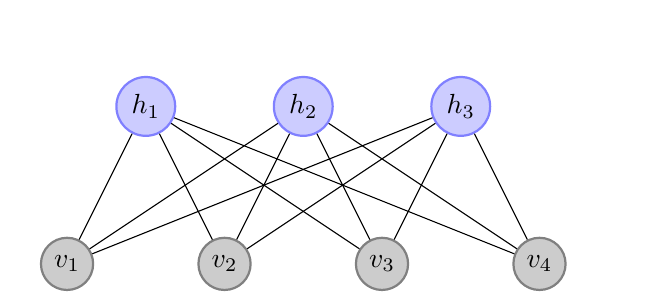
\begin{tikzpicture}
      [inner sep=1mm,
       hidden/.style={circle,draw=blue!50,fill=blue!20,thick},
       visible/.style={circle,draw=black!50,fill=black!20,thick}]
      \useasboundingbox (-0.5,0) rectangle (7,3);
      \node at (0,0) (v1) [visible] {$v_1$};
      \node at (2,0) (v2) [visible] {$v_2$};
      \node at (4,0) (v3) [visible] {$v_3$};
      \node at (6,0) (v4) [visible] {$v_4$};
      \node at (1,2) (h1) [hidden] {$h_1$};
      \node at (3,2) (h2) [hidden] {$h_2$};
      \node at (5,2) (h3) [hidden] {$h_3$};
      \foreach \x in {1,...,4}
         \foreach \y in {1,...,3}
           \draw [-] (v\x) to (h\y);
    \end{tikzpicture}
\end{center}

For a given RBM, we relate the units with the energy function as follow: 
    \[Energy(\textbf{v},\textbf{h}) = -\textbf{b}^{T}\textbf{h} - \textbf{c}^{T}\textbf{v}-\textbf{h}^{T}\textbf{W}\textbf{v}\] 
where $\textbf{b} \in \mathbb{R}^{H}, \textbf{c} \in \mathbb{R}^{V}$ are offset/bias vectors and $\textbf{W} \in \mathbb{R}^{H\times V}$ comprises the weights connecting units.

The joint probability $P(\textbf{v}, \textbf{h})$ is presented as follows:
    \[P(\textbf{v}, \textbf{h})=\frac{1}{Z}e^{-Energy(\textbf{v}, \textbf{h})}\] 
where $Z$ is the normalization term.

\subsection*{(a) Conditional probabilities $P(\textbf{v}|\textbf{h})$ and $P(\textbf{h}|\textbf{v})$ (2 pts)}
Assuming $\textbf{v}$ and $\textbf{h}$ are binary units, show $P(v_i=1 | \textbf{h})$ and $P(h_j = 1 | \textbf{v})$ are presented as follow:
\begin{align*}
    P(v_i=1|\textbf{h}) &= sigm(c_i + \textbf{h}^{T}\textbf{W}_{:,i})\\
    P(h_j=1|\textbf{v}) &= sigm(b_j + \textbf{W}_{j,:}\textbf{v})
\end{align*}
\noindent where $sigm(x) = \frac{1}{1 + e^{-x}}$.

\begin{soln}{height=\textheight}
% Put your answer here.  Please make sure you complete your answers within the given size of the box.
\end{soln}

\subsection*{(b) Free energy (3 pts)}
We obtain $P(\textbf{v})$ by marginalizing $\textbf{h}$ as follow:
    \[P(\textbf{v}) = \frac{\sum_{\textbf{h} \in \{0, 1\}^{H}} e^{-Energy(\textbf{v}, \textbf{h})}}{Z} = \frac{e^{-FreeEnergy(\textbf{v})}}{Z}\]
where $FreeEnergy(\textbf{v})$ form makes it easier to compute gradients with visible units only. 

When we rewrite the energy function as follow:
  \[Energy(\textbf{v}, \textbf{h})=-\beta(\textbf{v})-\sum_{j=1}^{H}\gamma_j(\textbf{v},h_j)\]

Show $P(\textbf{v})$ and $FreeEnergy(\textbf{v})$ could be presented as follow:
\begin{align*}
    P(\textbf{v}) &= \frac{e^{\beta(\textbf{v})}}{Z}\prod_{j=1}^{H}\sum_{h_j\in\{0, 1\}}e^{\gamma_j(\textbf{v}, h_j)} \\
    FreeEnergy(\textbf{v}) &=-\beta(\textbf{v})-\sum_{j=1}^{H}\log\sum_{h_j\in\{0, 1\}}e^{-\gamma_j(\textbf{v},h_j)} \\
    &= -\textbf{c}^{T}\textbf{v} - \sum_{j=1}^{H}\log\left(1 + e^{b_j + \textbf{W}_{j,:}\textbf{v}}\right)
\end{align*}

\begin{soln}{height=10cm}
% Put your answer here.  Please make sure you complete your answers within the given size of the box.
\end{soln}

\subsection*{(c) Log-likelihood gradient of $P(v)$ (5 pts)}
Show log-likelihood gradient of $P(v)$ could be presented as follows:
\begin{center}
    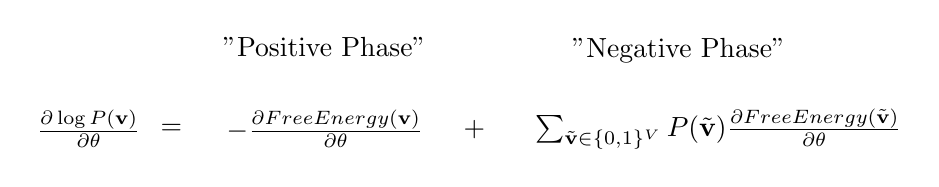
\begin{tikzpicture}[node distance=2cm]
      \node at (0,0) (a) {$\frac{\partial\log P(\textbf{v})}{\partial\theta}$};
      \node at (1.05,0) (b) {$=$};
      \node at (3,0) (c) {$-\frac{\partial FreeEnergy(\textbf{v})}{\partial\theta}$};
      \node at (4.9,0) (d) {$+$};
      \node at (8,0) (e) {$\sum_{\tilde{\textbf{v}}\in\{0,1\}^{V}}P(\tilde{\textbf{v}})\frac{\partial FreeEnergy(\tilde{\textbf{v}})}{\partial\theta}$};
      \node at (3,1.05) (f) {"Positive Phase"};
      \node at (7.5,1) (g) {"Negative Phase"};
    \end{tikzpicture}
\end{center}
Hint: present $\frac{\partial\log Z}{\partial\theta}$ in terms of $FreeEnergy(\textbf{v})$ and $P(\textbf{v})$.

\begin{soln}{height=10cm}
% Put your answer here.  Please make sure you complete your answers within the given size of the box.
\end{soln}

\subsection*{(d) Gradients with regard to each variables (5 pts)}

Show the gradients w.r.t. each variable $\textbf{W}, \textbf{b}, \textbf{c}$ could be presented as follows:
\begin{align*}
    -\frac{\partial\log P(\textbf{v})}{\partial W_{ji}} &= - P(h_j = 1|\textbf{v}) \cdot v_i + E_{\tilde{\textbf{v}}}[P(\tilde{h}_j = 1|\tilde{\textbf{v}})\cdot \tilde{v}_i] \\
    -\frac{\partial\log P(\textbf{v})}{\partial b_j} &= - P(h_j = 1 | \textbf{v}) + E_{\tilde{\textbf{v}}}[P(\tilde{h}_j = 1 | \tilde{\textbf{v}})] \\
    -\frac{\partial\log P(\textbf{v})}{\partial c_i} &= - v_i + E_{\tilde{\textbf{v}}}[\tilde{v}_i] \\
\end{align*}
Hint: use the results from (a).

\begin{soln}{height=10cm}
% Put your answer here.  Please make sure you complete your answers within the given size of the box.
\end{soln}

\subsection*{Contrastive Divergence}
In positive phase, we can compute the term with a training sample $\textbf{v}$. 
In negative phase, obtaining the expectation $E_{\tilde{\textbf{v}}}[\cdot]$ is intractable.
Contrastive Divergence replaces the expectation with a point estimate ($\tilde{\textbf{v}}, \tilde{\textbf{h}}$).
We obtain the point ($\tilde{\textbf{v}}, \tilde{\textbf{h}}$) by Gibbs sampling.
Given initial $\textbf{v}^{(0)}$, we sample $\textbf{h}^{(0)}\sim P(\textbf{h}|\textbf{v}^{(0)})$. Then we can sample $\textbf{v}^{(1)}\sim P(\textbf{v}|\textbf{h}^{(1)})$. 
After $k$ steps, we obtain $(\textbf{v}^{(k)},\textbf{h}^{(k)})$. 
As $k\rightarrow\infty$, sample $(\textbf{v}^{(k)},\textbf{h}^{(k)})$ are guaranteed to be accurate sample of $P(\textbf{v}, \textbf{h})$.
Then we can replace $E_{\tilde{\textbf{v}}}[P(\tilde{h}_j | \tilde{\textbf{v}})]$ with $P(h^{(k)}_j | \textbf{v}^{(k)})$.

\begin{center}
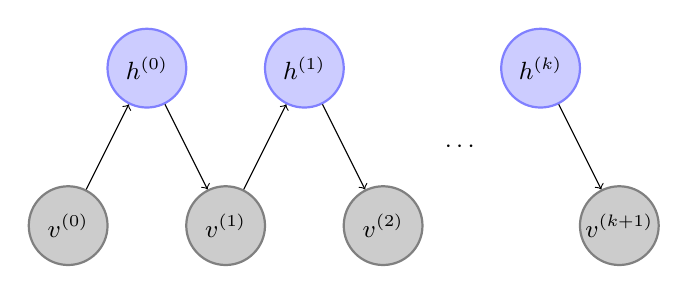
\begin{tikzpicture}
  [font=\small,
   inner sep=0pt,
   hidden/.style={circle,draw=blue!50,fill=blue!20,thick,minimum size=1cm},
   visible/.style={circle,draw=black!50,fill=black!20,thick,minimum size=1cm}]
  \node at (0,0) (v0) [visible] {$v^{(0)}$};
  \node at (1,2) (h0) [hidden]  {$h^{(0)}$};
  \node at (2,0) (v1) [visible] {$v^{(1)}$};
  \node at (3,2) (h1) [hidden]  {$h^{(1)}$};
  \node at (4,0) (v2) [visible] {$v^{(2)}$};
  \node at (6,2) (ht) [hidden]  {$h^{(k)}$};
  \node at (7,0) (vtt) [visible] {$v^{(k+1)}$};
  \draw [->] (v0) to (h0);
  \draw [->] (h0) to (v1);
  \draw [->] (v1) to (h1);
  \draw [->] (h1) to (v2);
  \draw [->] (ht) to (vtt);
  \node at (5,1) {$\cdots$};
\end{tikzpicture}
\end{center}

The initial sample in Gibbs sampling can be random values. 
Since we eventually want $P(\textbf{v})\approx P_{train}(\textbf{v})$, we start with a training example. 
Contrastive Divergence does not wait for the chain to converge. 
Only $k$-steps of Gibbs sampling is enough (so-called CD-$k$). 
$k=1$ has been shown to work surprisingly well in practice.

\subsection*{Deep Belief Network}
Top most layer is RBM. Others are directed belief networks.
\begin{center}
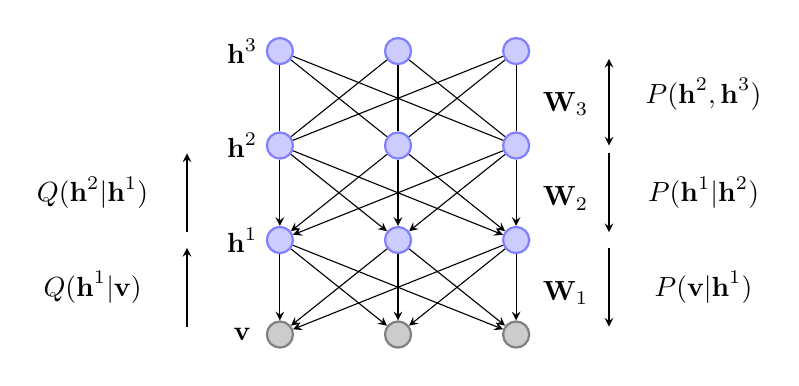
\begin{tikzpicture}
  \matrix (dbn)
   [matrix of math nodes,
    row sep={1.2cm,between origins},
    column sep={1.5cm,between origins},
    hidden/.style={circle,draw=blue!50,fill=blue!20,thick},
    visible/.style={circle,draw=black!50,fill=black!20,thick}]
   {
    |[hidden]|&|[hidden]|&|[hidden]|&\\
    |[hidden]|&|[hidden]|&|[hidden]|&\\
    |[hidden]|&|[hidden]|&|[hidden]|&\\
    |[visible]|&|[visible]|&|[visible]|&\\
   };
  \foreach \x [evaluate=\x as \ystart using int(\x+1)] in {2,3}
    \foreach \y in {\ystart}
      \foreach \a in {1,2,3}
        \foreach \b in {1,2,3}
          \draw [-stealth] (dbn-\x-\a) -- (dbn-\y-\b);
  \foreach \x in {1,2,3}
    \foreach \y in {1,2,3}
      \draw [-] (dbn-1-\x) -- (dbn-2-\y);
  \node at (dbn-2-3.north east) [xshift=5mm,yshift=4mm] {$\textbf{W}_3$};
  \node at (dbn-3-3.north east) [xshift=5mm,yshift=4mm] {$\textbf{W}_2$};
  \node at (dbn-4-3.north east) [xshift=5mm,yshift=4mm] {$\textbf{W}_1$};
  \node at (dbn-1-1.west) [xshift=-3mm] {$\textbf{h}^3$};
  \node at (dbn-2-1.west) [xshift=-3mm] {$\textbf{h}^2$};
  \node at (dbn-3-1.west) [xshift=-3mm] {$\textbf{h}^1$};
  \node at (dbn-4-1.west) [xshift=-3mm] {$\textbf{v}$};
  \draw [stealth-stealth] ([xshift=1cm,yshift=-1mm]dbn-1-3.east) to node [midway,xshift=12mm,yshift=1mm] {$P(\textbf{h}^2,\textbf{h}^3)$} ([xshift=1cm]dbn-2-3.east);
  \draw [-stealth] ([xshift=1cm,yshift=-1mm]dbn-2-3.east) to node [midway,xshift=12mm] {$P(\textbf{h}^1|\textbf{h}^2)$} ([xshift=1cm,yshift=1mm]dbn-3-3.east);
  \draw [stealth-] ([xshift=-1cm,yshift=-1mm]dbn-2-1.west) to node [midway,xshift=-12mm] {$Q(\textbf{h}^2|\textbf{h}^1)$} ([xshift=-1cm,yshift=1mm]dbn-3-1.west);
  \draw [-stealth] ([xshift=1cm,yshift=-1mm]dbn-3-3.east) to node [midway,xshift=12mm] {$P(\textbf{v}|\textbf{h}^1)$} ([xshift=1cm,yshift=1mm]dbn-4-3.east);
  \draw [stealth-] ([xshift=-1cm,yshift=-1mm]dbn-3-1.west) to node [midway,xshift=-12mm] {$Q(\textbf{h}^1|\textbf{v})$} ([xshift=-1cm,yshift=1mm]dbn-4-1.west);
\end{tikzpicture}
\end{center}

\textbf{DBN training}: We will use the layer-wise training algorithm. Namely, we first learn an RBM with an input layer $\textbf{v}$ and a hidden layer $\textbf{h}^{1}$, then freeze this RBM. 
We generate new training data $\textbf{h}^{1}$ by sampling $p(\textbf{h}^{1}|\textbf{v})$ for every $\textbf{v}$ in the training set (one per sample in the training set), and use this as the input to the second RBM ($\textbf{h}^{1}$ and $\textbf{h}^{2}$). 
The third RBM ($\textbf{h}^{2}$ and $\textbf{h}^{3}$) is also trained in this way.

\textbf{DBN generation}: After training a DBN, we could sample a vector $\textbf{h}^{2}$ using Gibbs sampling from the third RBM.
Given initial $\textbf{h}^{2^{(0)}}$, we sample $\textbf{h}^{3^{(0)}}\sim P(\textbf{h}^{3}|\textbf{h}^{2^{(0)}})$. 
Then we can sample $\textbf{h}^{2^{(1)}}\sim P(\textbf{h}^{2}|\textbf{h}^{3^{(0)}})$. 
After $k$ steps, we obtain $\textbf{h}^{2^{(k)}}$.
Then, using $\textbf{h}^{2^{(k)}}$, we sample lower layers, $\textbf{h}^{1}$ followed by $\textbf{v}$, using sigmoid belief networks.

\pagebreak

\clearpage
\section*{Programming (60 pts)}
Two files, \texttt{rbm.py} and \texttt{dbn.py}, are provided. 
Only \texttt{rbm.py} will be evaluated in autograder, but you need to implement both to answer all questions below. 
You should read the instructions on top of these files, and the docstrings very carefully. 
You can change anything as you see fit in \texttt{dbn.py}, as this file will not be autograded. 
\textbf{Zip only \textit{rbm.py} file and upload the zip file to GradeScope as shown in Figure~\ref{fig:submission_example}.}

\begin{figure}[H]
\centering
\includegraphics[width=.35\linewidth]{images/programming_1.png}
\caption{Submission Example.} 
\label{fig:submission_example}
\end{figure}

As assistance through the programming assignment, we provided access to the \textcolor{blue}{hw2.ipynb} jupyter notebook, where the paths and dependencies are managed. The final submission will still be this pdf.

\vspace{10mm}
In this assignment, the reconstruction error refers to:
\begin{equation}
    \frac{1}{N}\sum_{i=1}^{N}\sqrt{\sum_{j=1}^{m}(x_{ij}-\tilde{x}_{ij})^{2}}
\end{equation}
where N is the number of samples in training set or validation set, m is the dimension of data vector, $x$ is the input vector and $\tilde{x}$ is the reconstructed vector. Perform Gibbs sampling with $k=1$ to obtain $\tilde{x}$. 

We will build and train generative models (RBM and DBN) for MNIST dataset, which are images of 10 handwritten numbers. The images are 28 by 28, but they will be represented as 1D vectors with length 784. Data for training, validation and testing can be found in \texttt{digitstrain.txt}, \texttt{digitsvalid.txt}, and \texttt{digitstest.txt}.

For training, choose a reasonable learning rate (e.g. 0.1 or 0.01) and use your own judgement to decide when to stop training (i.e number of epochs or convergence criteria). 


\clearpage
\subsection*{1. RBM task}
Initialize an RBM with 100 hidden units. 

\paragraph{a.1)} \textbf{Autograder (20 points)}

This question only requires your \texttt{rbm.py} Autograder submission.

\paragraph{a.2)} \textbf{Training(5 points)}

Try the RBM model with gibbs steps $k$ as 1, 3, and 5. For each $k$, plot reconstruction error against the epoch number for training and validation on one plot. So you should include 3 plots here, each contains two curves for training and validation. How does $k$ affect training convergence of the model?

\begin{soln}{height=5cm}
% Put your answer here.  Please make sure you complete your answers within the given size of the box.
\end{soln}

\paragraph{b)} \textbf{Visualizing and understanding learned parameters (5 points)}

Choose one model that you like, and visualize its learned $W$ as 100 images that are 28-by-28 in pixel. Plot all of them in one figure. What are being plotted here? Do they exhibit any structure?

\begin{soln}{height=5cm}
% Put your answer here.  Please make sure you complete your answers within the given size of the box.
\end{soln}

% \paragraph{c) Reconstruction} \textbf{(10 points)}

% To qualitatively test the model performance, plot 100 pairs of original and reconstructed images as comparison. 
% To reconstruct, feed a real sample from test set into the model as visible vector, generate a new sample for visible vector as the reconstruction by 1 step of gibbs sampling. 
% % Plot 50 pairs of original and reconstructed images, which are 100 images, in 10 lines in total, with 5 pairs each line. 
% % On the 1st line, plot 5 pairs for the digit \textbf{1}, and digit \textbf{2} for the 2nd line, etc. 

% \begin{tcolorbox}[fit,height=4cm, width=16cm, blank, borderline={1pt}{-2pt},nobeforeafter]
% \begin{soln}
% \end{soln}
% \end{tcolorbox}

\paragraph{c) Generation} \textbf{(5 points)}

Set $k>1000$ for this task. Display the 100 generated samples for digit images in one figure. Do they look like handwritten digits? What if you retrain your RBM on only 3 digits, say $\textbf{1, 2}$ and $\textbf{3}$? If you train with $k=1$ vs $k=5$, do you see a difference in generated figures?

\begin{soln}{height=5cm}
% Put your answer here.  Please make sure you complete your answers within the given size of the box.
\end{soln}

\paragraph{d) Conditional generation} \textbf{(5 points)}

Only reveal the top half of MNIST images (data generation code is provided to you), and use the RBM to reconstruct the bottom half of the image. Note here when you do gibbs sampling, when you sample $\bf v$ condition on $\bf h$, part of $\bf v$ is known for sure. You need to inject these known value to the newly sampled $\bf v$. 

\begin{soln}{height=5cm}
% Put your answer here.  Please make sure you complete your answers within the given size of the box.
\end{soln}

\paragraph{e) Supervised learning with RBM} \textbf{(10 points)}

Take the RBM you have trained and initialize a 2-layer neural network, of which the first layer's weights are initialized using the RBM's weight. Compare the training trajectory of this RBM-initialized network with a randomly initialized network. Does the RBM-initialized network converge faster? Plot the training loss of these two networks in one figure.

\begin{soln}{height=5cm}
% Put your answer here.  Please make sure you complete your answers within the given size of the box.
\end{soln}


\subsection*{2. DBN task}
Truncate our dataset and only retain images of digits \textbf{7}, \textbf{8}, and \textbf{9}.
Build a DBN with two hidden layers with 500 and 784 units respectively, so there are two RBMs with 500 and 784 hidden units. 

\paragraph{a) Training} \textbf{(5 points)}
Training this DBN with gibbs steps $k=3$. For each RBM, plot reconstruction error against the epoch number for training and validation on one plot. So you should include 2 plots here, each contains two curves for training and validation.

\begin{soln}{height=5cm}
% Put your answer here.  Please make sure you complete your answers within the given size of the box.
\end{soln}

\paragraph{b) Generation} \textbf{(5 points)}

Set $k>1000$ for this task. Display the 100 generated samples for digit images in one figure. Do they look like handwritten digits? 

\begin{soln}{height=5cm}
% Put your answer here.  Please make sure you complete your answers within the given size of the box.
\end{soln}
\clearpage
\input{collaboration.tex}
\clearpage

\end{document}